\section{from light to electron}
Human have long history of harnessing light and creating optical microscopes that allow us to look closer. The resolution of the microscope is physically limited by the wavelength of the light, as framed by Abbe's diffraction limit:
\begin{equation}
	d = \frac{\lambda}{2\cdot NA}.
\end{equation}
This states that the smallest distance $d$ at which two points can be distinguished as separate is approximately half of the wavelength of light being used, modified by the numerical aperture $NA$ of the objective lens. This means for a visible light of $\lambda \approx 500nm$, the best possible resolution is around $200$ to $250nm$. By developing light sources with shorter wavelength, scientists were able to push the optical boundary. With the development of UV microscopy in the 1920s, the spatial resolution was pushed to approximately $100nm$. 

People start to look for something with shorter wavelength to resolve finer structures. According to the matter wave theory proposed by Louis de Broglie in 1924, matter exhibits wave-like behavior with a wavelength $\lambda$ inversely proportional to its momentum $p$: 
\begin{equation}
	\lambda = \frac{h}{p},
\end{equation}
where $p$ is the Planck constant. 

This inspired people to look into electrons, whose wavelength is orders of magnitude smaller than that of light, and whose momentum is easier to manipulate through electric field. Ernest Ruska made the most important foundational contributions to electron optics and designed the first electron microscope in 1930s. Borrowing the same set up in a conventional microscope, Ruska designed a transmission electron microscope(TEM), by letting the electron beam piercing through a thin section of the object. The invention of TEM brought the resolution to about $10nm$, achieving the best resolution at that time. 

Scanning tunneling microscope(STM) marks another attempt to manipulate electrons for high-resolution imaging. However, it is not a true microscope that gives a direct image of an object; instead, it is more like how a blind person reads the Braille as shown in Figure \ref{fig:braille} panel a). Similar to how fingers detect the impressed characters, \ac{STM} scans a metallic tip to "sense" the structure of a sample surface, as illustrated in pane b). However, the sensing is not down by making mechanical contact, instead, an \ac{STM} tip is placed very closed(\textasciitilde $1nm$) to the sample surface and by applying a bias voltage across the tip-sample junction, electrons from one side will travel through the vacuum barrier to the other side, creating a current. The principle enabled this counter intuitive movement of electron across the vacuum barrier is called quantum tunneling effect, hence the name of the instrument. The first \ac{STM} was introduced by Gred Binnig and Heinrich Rohrer in 1981. Next year in 1982, Binnig and Rohrer performed the first surface topography with this new-born; they inspected the surface of Si(111) and observed the $7 \times 7$ reconstruction as shown in Figure \ref{figure:si111_binnig}\cite{binnig77Reconstruction1983}. This direct observation of the 12 adatoms in a unit cell allows them to propose a modified model for the adatoms. With the invention and development of \ac{STM}, scientists for the first time, were able to visualize and manipulate atomic features with a picometer($10^{-12}$m) resolution.
\begin{figure}
	\centering
	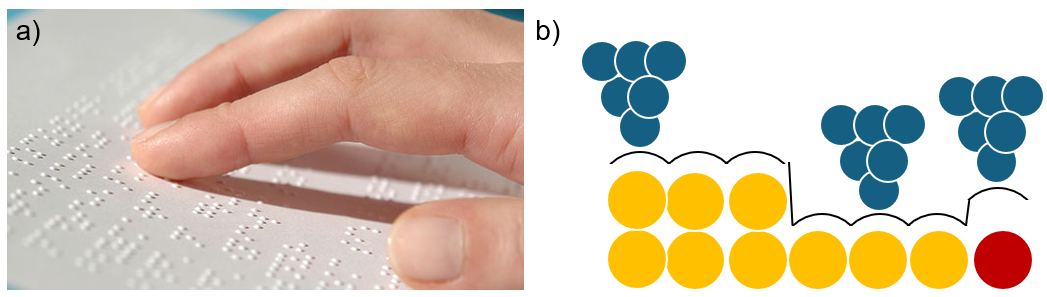
\includegraphics[width=0.8\textwidth]{braille.png}
	\caption{Analogy between the Braille reading and STM topography}
	\label{fig:braille}
\end{figure}
The foundational work done by Ruska, Binnig and Rohrer on electron microscope was awarded the 1986 Nobel Price in Physics. From the earliest optical instruments to the advent of electron-based probes, each leap in resolution has revealed new structural detail. STM represents the culmination of this progression, pushing beyond the limits of conventional electron optics by harnessing quantum tunneling rather than direct imaging. With its ability to map surfaces atom by atom, STM opens up entirely new fields, including the study of point defects in quantum materials

\begin{figure}
	\centering
	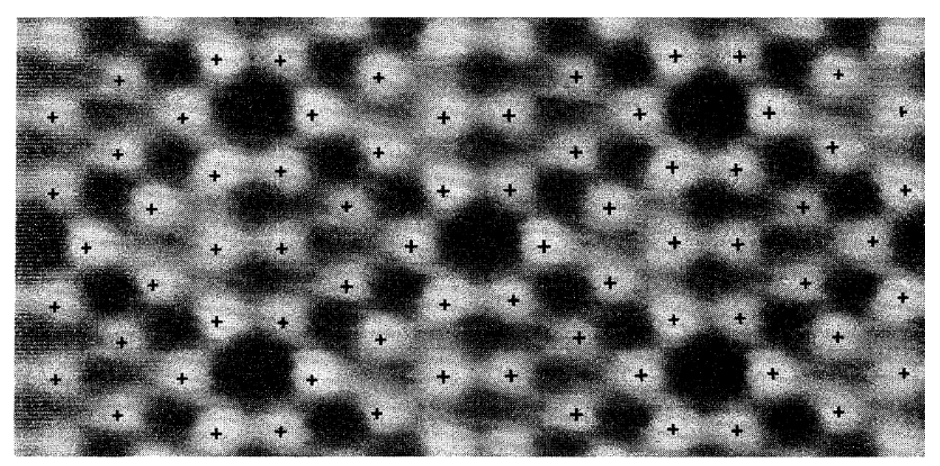
\includegraphics[width=0.8\textwidth]{Si111_binnig.png}
	\caption{}
	\label{figure:si111_binnig}
\end{figure}

In this chapter, we will first explain the theory of \ac{STM}, then introduce the configuration of a modern \ac{STM}, and close with an introduction on the instrument we used for this study. 

\section{Theory of STM}
In essence, an \ac{STM} works by collecting and analyzing the tunneling current between the tip and sample. Thus, the quantitative understanding of the tunneling current is the core of theory of \ac{STM}, and thus the focus of this section. We will first give a overview on the quantum tunneling and the theory development in history, then we will elaborate on the derivation of tunneling current in a typical tip-sample geometry.

\subsection{quantum tunneling and development of STM theory}
Quantum tunneling described the behavior of quantum mechanical object passing through a potential barrier that is higher than their energy. The word passing through is adopting the classical particle point of view, for a quantum mechanical object that exhibit wave-particle duality, we should say that the wave function of this object has a finite amplitude on the other side of the barrier, and thus a non-zero probability density to find the object in the classically prohibited region. Quantitatively, according to the WKB approximation, the transmission probability $T$ for a particle with mass $m$ and energy $E$, given a potential barrier of $V$ with width $\alpha$ is: 
\begin{equation}
	T \approx e^{-\alpha\sqrt{\frac{8m}{\hslash^2}(V-E)}}. 
\end{equation}
In fact, according to de Broglie's  matter wave theory, even a classical object could theoretically tunnel through a seemly forbidden barrier, just extremely unlikely: the probability for a baseball traveling at 40 m/s to tunnel through a 10 cm thick brick wall is approximately $e^{-10^{33}}$. 

The development of theory of quantum tunneling can be dated in 1928, when Robert Oppenheimer developed a time-dependent perturbation method trying to explain the ionization of hydrogen in an apply field\cite{oppenheimerThreeNotesQuantum1928}. A more general theory for a metal-insulator-metal junction is introduced by Bardeen in 1961\cite{bardeenTunnellingManyParticlePoint1961}, 20 years before the birth of \ac{STM}. Two years after the invention of \ac{STM}, Tersoff and Hamann extended Bardeen's theory to model an ideal STM tip-sample junction, which successfully interpreted the topography of Au crystal \cite{tersoffTheoryApplicationScanning1983}\cite{tersoffTheoryScanningTunneling1985}. Later, Lang found that one can effectively model the \ac{STM} operation with tunneling between only the single atom on the end of a tip(the acting atom) and the single atom on the surface, revealing the atomic nature of the \ac{STM} \cite{langVacuumTunnelingCurrent1985}\cite{langSpectroscopySingleAtoms1986}\cite{langApparentSizeAtom1987}. Inspired by the atomic picture, Julian Chen built a three-dimensional model of the tunneling considering different tip configurations by expanding the asymptotic wave function of the acting atom\cite{chenTunnelingMatrixElements1990}\cite{chenTheoryScanningTunneling1988}. 

Since our work include using a simple tungsten tip and a low bias voltage(amplitude within 1V), it is sufficient to use the result from Teroff and Hamann.  

\subsection{Tunneling current--from Bardeen to Tersoff and Hamann}
According to Fermi's golden rule, the transmission probability between the tip and sample is directly related to the matrix element $M_{ts}$ between the tip's state $\psi_{t}$, sample's state $\psi_{s}$, and their corresponding electron density $\rho$. When applied a small bias voltage $V_s$ to the sample, we can write:
\begin{align}
	P_{t->s} &= \frac{2\pi}{\hslash}\int_{-\infty}^{\infty}|M_{ts}|^2\rho_s(\epsilon + eV_s)[1-f(\epsilon+eV_s)]\cdot \rho_t(\epsilon)f(\epsilon) d\epsilon \\
	P_{s->t} &= \frac{2\pi}{\hslash}\int_{-\infty}^{\infty}|M_{ts}|^2\rho_s(\epsilon + eV_s)f(\epsilon+eV_s)\cdot \rho_t(\epsilon)[1-f(\epsilon)] d\epsilon,
\end{align} 
where $f$ represents the Fermi-Dirac function. It is worth noting that in order to use Fermi's golden rule, an equilibrium condition is assumed; this is generally satisfied as the internal relaxation time scale for metallic electrodes are in the range of femtosecond to picosecond, which is much smaller than milliseconds settling time used in standard \ac{STM} measurements. 

The tunneling current proportional to the net transmission probability across tip and sample, under one key assumption: the tunneling must not change the occupation number of both the sample and tip side. This is generally true since the tunneling current is normally is the order of nano-Ampere to pico-Ampere; this correspond to approximately $10^6 \textasciitilde 10^9$ electrons per second, which is tiny compared to the total number of electrons in both electrodes. Thus we can write the tunneling current $I_t$:
\begin{align}
	I_t & = 2e(P_{t->s}-P{s->t})\\
	& = 2e \cdot \frac{2\pi}{\hslash}\int_{-\infty}^{\infty}|M_{ts}|^2\rho_t(\epsilon) \rho_s(\epsilon + eV_s) \cdot[f(\epsilon) - f(\epsilon + eV_s)] d\epsilon.
\end{align}
The factor of 2 is a result of the spin degeneracy. At low temperature, when $k_BT<<V_s$, we can replace the Fermi-Dirac distribution function $f$ with a step-wise function, and simplifies the integral to: 
\begin{equation}
	\label{eq:I_t}
	I_t = \frac{4e\pi}{\hslash}\int_{0}^{eV_s}|M_{ts}|^2\rho_t(\epsilon - eV_s) \cdot \rho_s(\epsilon)d\epsilon. 
\end{equation} 
From Equation \ref{eq:I_t}, we note that the tunneling current is proportional to both $\rho_t$ and $\rho_s$, since we are interested in probing the sample, we can simply pick the tip to have a featureless $\rho_t$. This can be achieved by using simple metal and their alloys; typically, \ac{STM}s today use tips made of tungsten or a platinum-iridium.

The matrix element can be intuitively understood as the overlapping of sample states and tip states within the insulating barrier. Analytically, it can be expressed as: 
\begin{equation}
	content...
\end{equation}

However, the analytical determination of this overlap turns out to be a very difficult problem, especially when the tip and sample electronic geometries are unknown. The understanding of the matrix element that I will present was two stepped. First, Bardeen made a leap forward by crafting a general expression with a few assumptions given; then Tersoff and Hamann applied it to the ideal configuration of an STM, with a sharp tip and a flat sample surface. I will not elaborate the details of Bardeen's monstrous derivation on the general expression, and if the readers are curious, a very comprehensive and accessible tutorial can be found here\cite{gottliebBardeensTunnelingTheory}. I will, however, elaborate Tersoff and Hamann's work, but with a better proof proposed by Julian Chen \cite{chenTunnelingMatrixElements1990}, as the corresponding result sets the theoretical foundation for \ac{STM}'s key capacity as a local probe.  

a situation that  with a lot of assumptions and is a beast on its own. Intuitively, it is the  And area that I will not elaborate is  Matrix element between the tip and sample was initially formulated by Bardeen as: 
\begin{equation}
	M_{ts}^{\mu\nu} = \frac{\hslash^2}{2m}\int_{\Sigma}[\psi_s^{\mu}\nabla\psi_t^{\nu*} - \psi_t^{\mu*} \nabla \psi_s^{\nu}]\cdot d\mathbf{S},
\end{equation}
where $\psi_s^{\mu}$ and $\psi_t^{\nu}$ are the sample and tip wave functions at energy $E_\mu$ and $E_\nu$, respectively. The whole integral is down on the  


In Bardeen's tunneling theory, he considered a metal-insulator-metal junction. Since we will eventually extend it to \ac{STM}, we can name the metal on the left side as Tip $T$, and other side as sample $S$. Initially, the two    
\begin{figure}
	\centering
	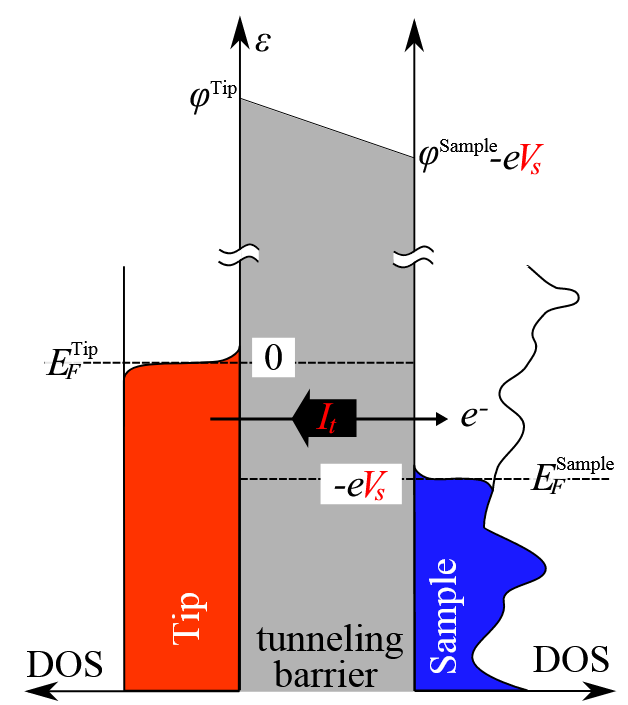
\includegraphics[width=0.8\textwidth]{tunneling_schematic.png}
	\caption{}
	\label{fig:tunneling}
\end{figure}
Quantum tunneling is what allows \ac{STM} to probe surfaces without making mechanical contact. 


\section{Configuration of an STM}

A schematic of an \ac{STM} is shown in \ref{fig:stm_schematics}, 

\begin{figure}
	\centering
	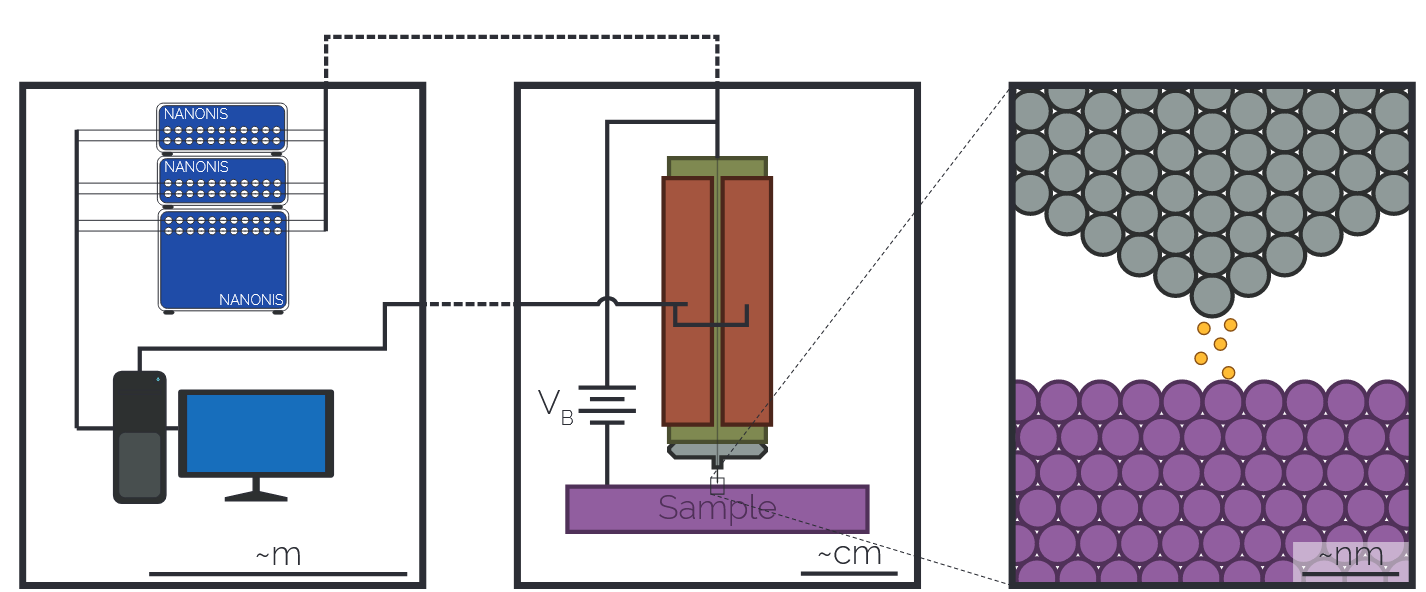
\includegraphics[width=0.8\textwidth]{STM_schematic.png}
	\caption{}
	\label{fig:stm_schematics}
\end{figure}